% === START TEMPLATE WITH CONFIGURABLE WATERMARK POSITION ===
\documentclass[10pt]{article}
\usepackage[utf8]{inputenc}
\usepackage[left=50pt,right=50pt,top=100pt,bottom=100pt]{geometry}
\usepackage[T1]{fontenc}
\usepackage{lmodern}
\usepackage[hidelinks]{hyperref}
\usepackage{graphicx}
\usepackage[table]{xcolor}
\usepackage{transparent}
\usepackage{tabularx}
\usepackage{stackengine}
\usepackage{mwe}
\usepackage{tocloft}
\usepackage[hypcap=false,font=small]{caption}
\usepackage{capt-of}
\usepackage{multicol}
\usepackage{ragged2e}
\usepackage{titlesec}
\usepackage{fancyhdr}
\usepackage{etoolbox}
\usepackage{eso-pic}

% === User-Configurable Variables ===
\newcommand{\ProductName}{ILM139C RGB LED Matrix}
\newcommand{\ProductNameShort}{ILM139C}
\newcommand{\WebsiteLinkText}{www.rudectech.com}
\newcommand{\ReleaseDate}{2025-05-13}
\newcommand{\Revision}{Rev.\ 1.0}

% === Watermark Variables ===
\newcommand{\WatermarkPath}{example-image}
\newcommand{\WatermarkScale}{0}
\newcommand{\WatermarkAngle}{45}
\newcommand{\WatermarkOpacity}{0.1}
\newcommand{\WatermarkPosX}{0.1\paperwidth}
\newcommand{\WatermarkPosY}{0.1\paperheight}

% Place watermark
\AddToShipoutPictureBG{%
	\AtPageLowerLeft{%
		\raisebox{\WatermarkPosY}[0pt][0pt]{%
			\makebox[\WatermarkPosX][l]{%
				\transparent{\WatermarkOpacity}%
				\includegraphics[scale=\WatermarkScale,angle=\WatermarkAngle]{\WatermarkPath}%
			}%
		}%
	}%
}

% TOC config
\renewcommand{\contentsname}{Table of Contents}
\setcounter{tocdepth}{2}
\renewcommand{\cftdotsep}{1.5}
\renewcommand{\cftsecleader}{\cftdotfill{\cftdotsep}}
\renewcommand{\cftsubsecleader}{\cftdotfill{\cftdotsep}}
\setlength{\cftbeforesecskip}{0.5em}
\setlength{\cftbeforesubsecskip}{0.5em}

\renewcommand{\familydefault}{\sfdefault}

\pagestyle{fancy}
\fancyhf{}
\renewcommand{\headrulewidth}{0.4pt}
\renewcommand{\footrulewidth}{0.4pt}
\setlength{\headheight}{60pt}
\setlength{\headsep}{10pt}
\setlength{\footskip}{50pt}
\lhead{
\includegraphics[height=0.8cm]{../visual/badges/illumicro_logo.png}}
\rhead{%
	
\includegraphics[height=0.6cm]{../visual/badges/edrtech_logo.png}\\[-0.5em]
	{\scriptsize\textcolor{gray!50}{\WebsiteLinkText}}%
}
\fancyfoot[L]{\footnotesize\textcolor{gray!50}{{\ProductNameShort} Datasheet}}%
\fancyfoot[C]{\footnotesize\textcolor{gray!50}{\Revision}}
\fancyfoot[R]{\footnotesize\textcolor{gray!50}{\thepage}}

\fancypagestyle{plain}{%
	\fancyhf{}%
	\lhead{\Large\textbf{\ProductNameShort}}%
	\rhead{%
		
\includegraphics[height=0.6cm]{../visual/badges/edrtech_logo.png}\\[-0.5em]
		{\scriptsize\textcolor{gray!50}{\WebsiteLinkText}}%
	}%
\fancyfoot[L]{\footnotesize\textcolor{gray!50}{{\ProductNameShort} Datasheet}}%
	\fancyfoot[C]{\footnotesize\textcolor{gray!50}{\Revision}}%
	\fancyfoot[R]{\footnotesize\textcolor{gray!50}{\thepage}}%
	\renewcommand{\headrulewidth}{0.4pt}%
	\renewcommand{\footrulewidth}{0.4pt}%
}

\setcounter{secnumdepth}{3}
\renewcommand{\thesubsection}{\arabic{section}.\arabic{subsection}}
\renewcommand{\thesubsubsection}{\arabic{section}.\arabic{subsection}.\arabic{subsubsection}}
\titleformat{\subsection}[hang]
{\large\bfseries}{\thesubsection}{1em}{}
[\color{gray!30}\rule{\textwidth}{0.4pt}]
\titlespacing*{\subsection}{0pt}{1.5\baselineskip}{1\baselineskip}
\newcommand{\sectionbreak}{\clearpage}

\begin{document}
	\flushbottom
	\begin{center}
		{\LARGE\bfseries \ProductName\par}
		\vspace{1ex}
		{\normalsize Datasheet\par}
	\end{center}
	\vspace{2\baselineskip}
	
	\noindent
	\begin{minipage}[t]{0.45\textwidth}
		\section{Features}\label{sec:features}
		\vspace{\baselineskip}
		\begin{itemize}
			\item 13x9 RGB LED matrix
			\item Small 26mm*18mm Footprint
			\item 2mm pitch, 1mm x 1mm LEDs
			\item Based on IS31FL3741A LED driver
			\item Individual LED PWM control
			\item 2.7V–5.5V input voltage range
			\item Qwiic-compatible connector
			\item Optional 2-pin power connector
			\item I\textsuperscript{2}C address selection via jumpers
		\end{itemize}
	\end{minipage}
	\hfill
	\begin{minipage}[t]{0.5\textwidth}
		\section{Description}\label{sec:desc}
		\vspace{\baselineskip}
		This compact RGB LED matrix module integrates a high-density 13×9 full-color LED array with an onboard IS31FL3741 driver IC. Designed for seamless integration into I2C-based systems, the module supports individual PWM control of all 351 LEDs and features a robust, stackable form factor suitable for embedded, wearable, and interactive display applications.
		
	\begin{center}
		\vskip 30px
	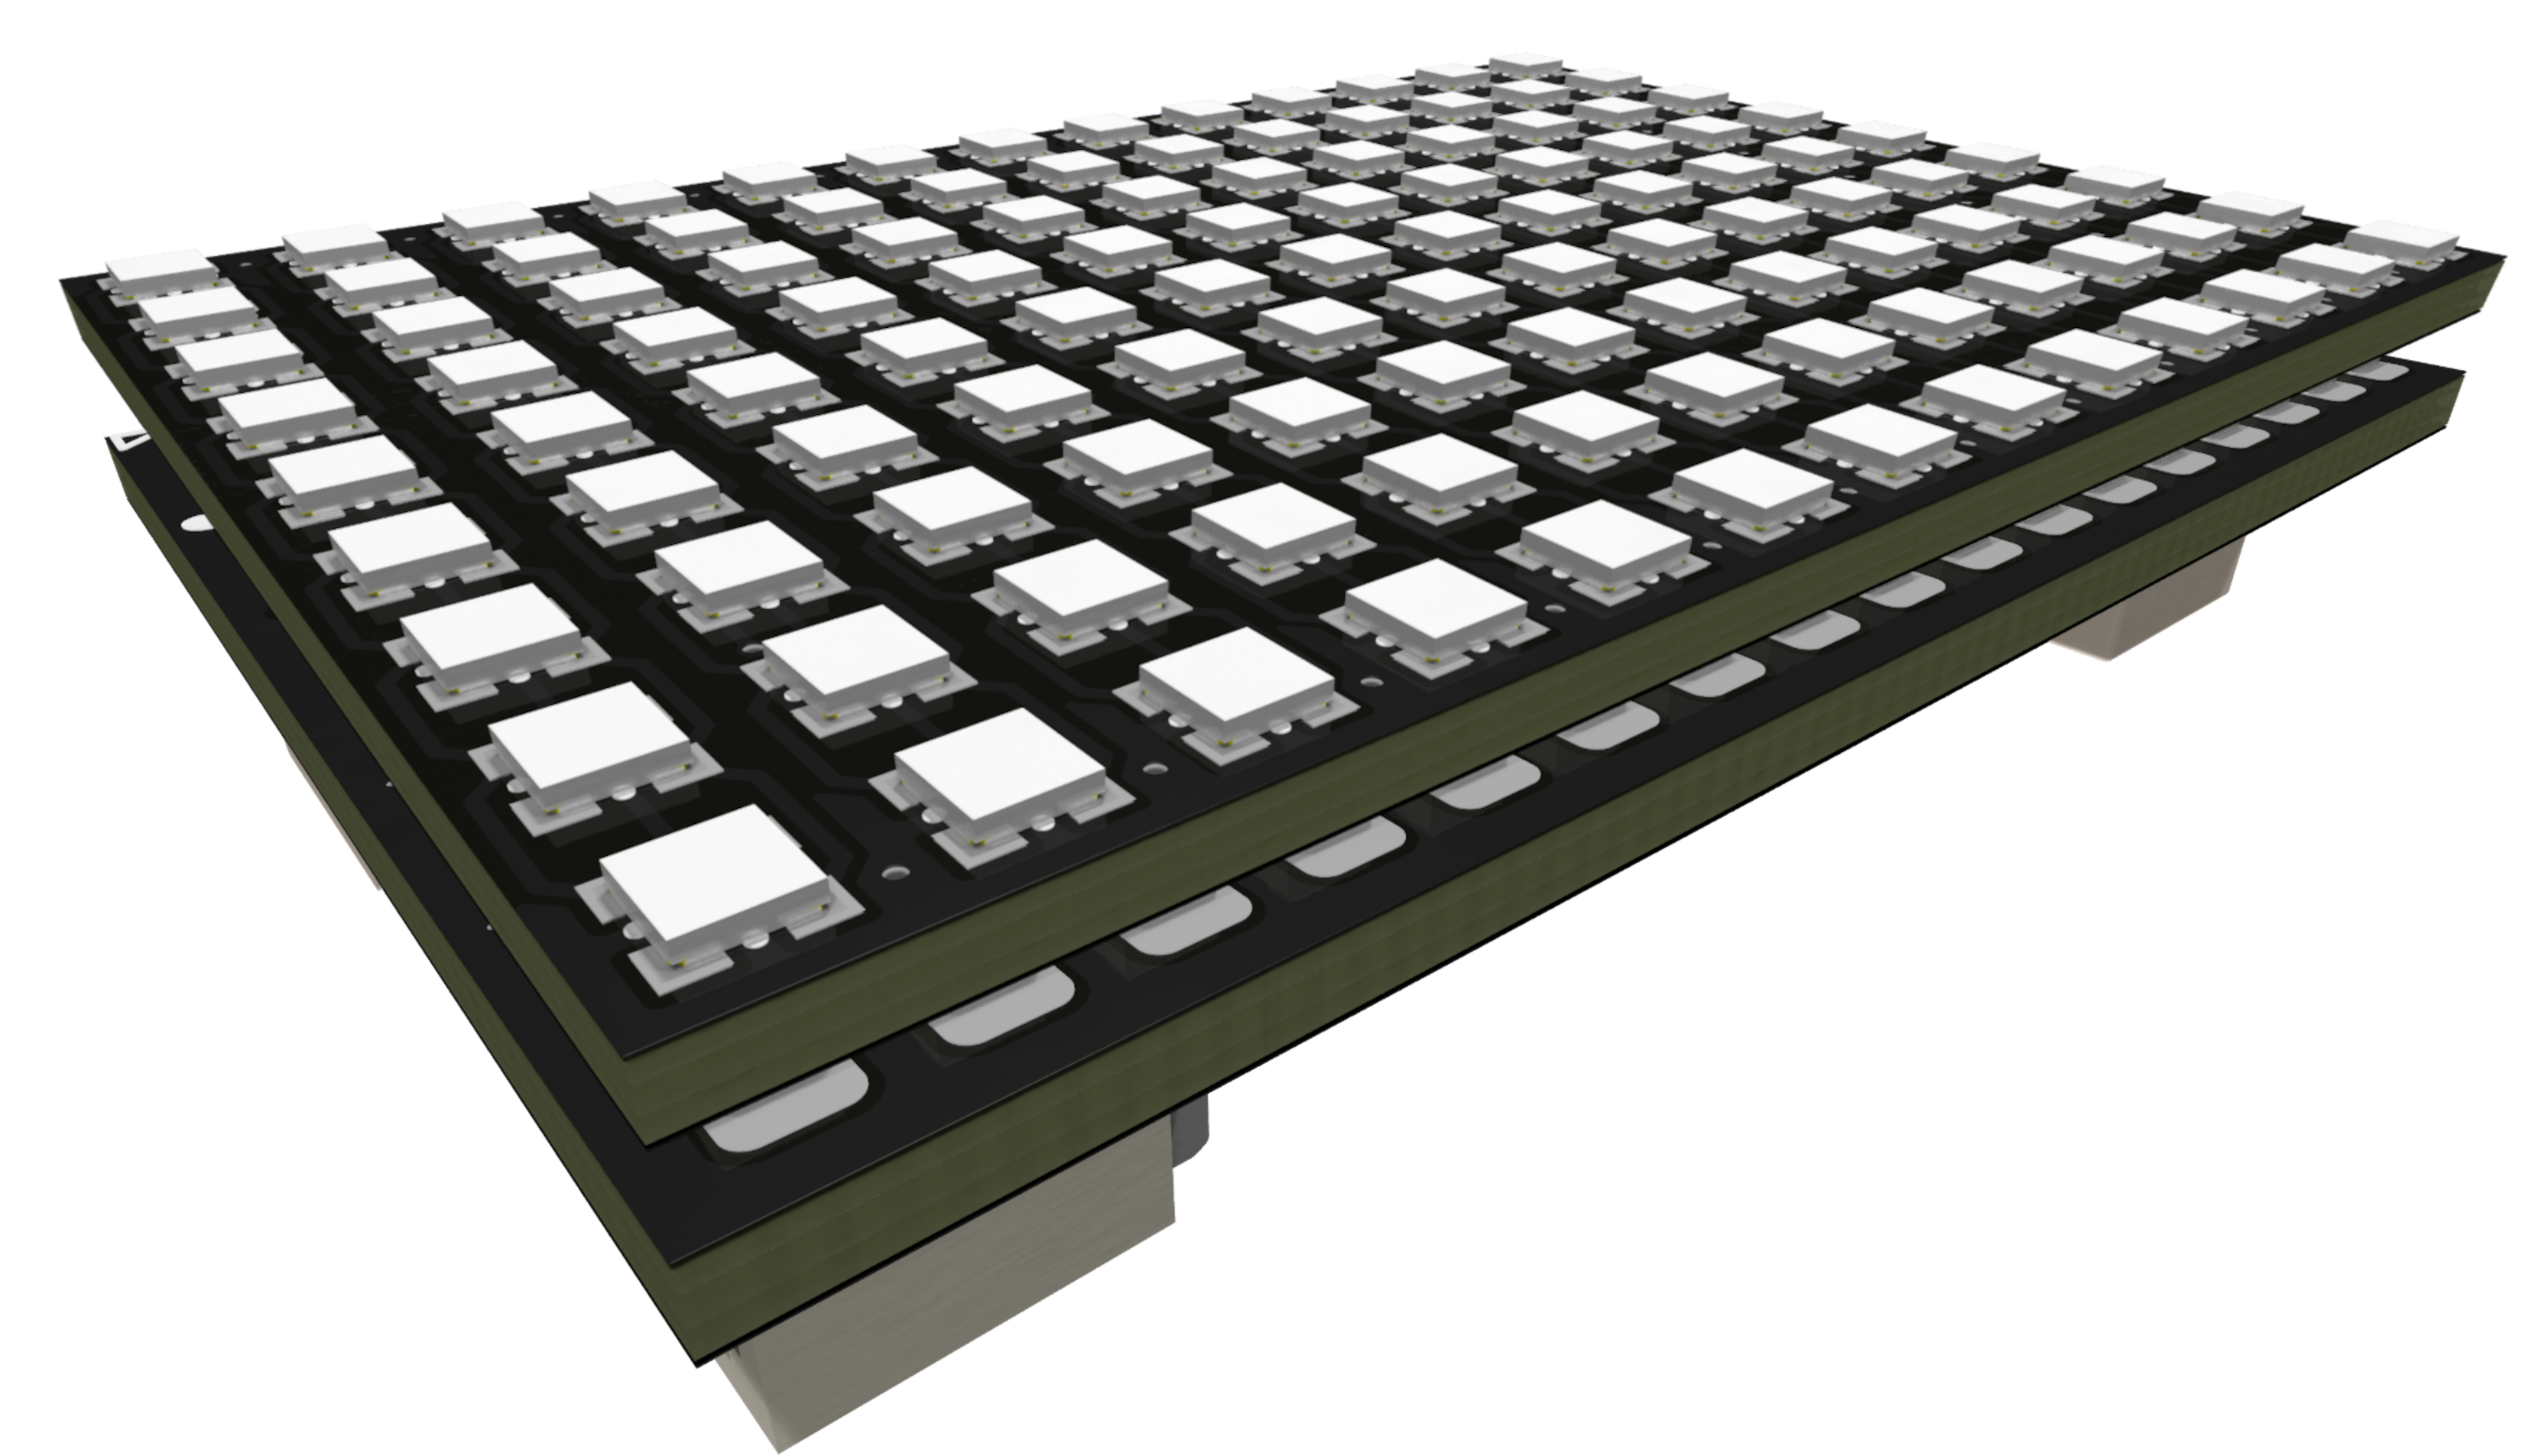
\includegraphics[width=150px]{../visual/ILM139C_iso_3d.png}
	\captionof{figure}{Module Overview}
	\label{fig:component}
\end{center}

	\end{minipage}
	
	\section*{\contentsname}
	\begin{multicols}{2}
		{\let\oldcontentsname\contentsname
			\renewcommand{\contentsname}{}
			\tableofcontents
			\let\contentsname\oldcontentsname}
	\end{multicols}
	
	\vspace{1em}
	\noindent\textbf{Revision History}\par
	\begin{tabularx}{\textwidth}{|l|X|}
		\hline
		\rowcolor{gray!25}\textbf{Date} & \textbf{Description} \\ \hline
		\ReleaseDate & Initial release \\ \hline
	\end{tabularx}
	\captionof{table}{Revision History}\label{tab:rev}
	
	\sectionbreak
	
	\section{Device Overview}\label{sec:overview}
	\subsection{Part Number Options}\label{sec:overview.1}
	\begin{tabularx}{\textwidth}{|X|X|X|}
		\hline
		\rowcolor{gray!25}\textbf{PART NUMBER} & \textbf{PACKAGE} & \textbf{DESCRIPTION} \\ \hline
		ILM139C & 26mm × 18mm × 3.2mm & Complete module \\ \hline
		ILM139CD & Driver board & IS31FL3741A module \\ \hline
		ILM139CM & LED matrix board & 13x9 RGB LED matrix module \\ \hline
	\end{tabularx}
	\captionof{table}{Part Number Options}\label{tab:overview1}
	\sectionbreak
	\subsection{Pin Configuration and Functions}\label{sec:overview.2}
	\begin{tabularx}{\textwidth}{|l|X|}
		\hline
		\rowcolor{gray!25}\textbf{Label} & \textbf{Description} \\ \hline
		SDA & I\textsuperscript{2}C data \\ \hline
		SCL & I\textsuperscript{2}C clock \\ \hline
		INT & Interrupt output \\ \hline
		SDB & Shutdown \\ \hline
		3.3V & QWIIC 3.3V \\ \hline
		VCC & 2.7V~5.5V Power supply input \\ \hline
		GND & Ground \\ \hline
		3.3V->VCC Jumper & 0603 SMD Jumper. If present, VCC=QWIIC 3.3V \\ \hline
	\end{tabularx}
	\captionof{table}{Pin description}\label{tab:rev}
	\begin{center}
		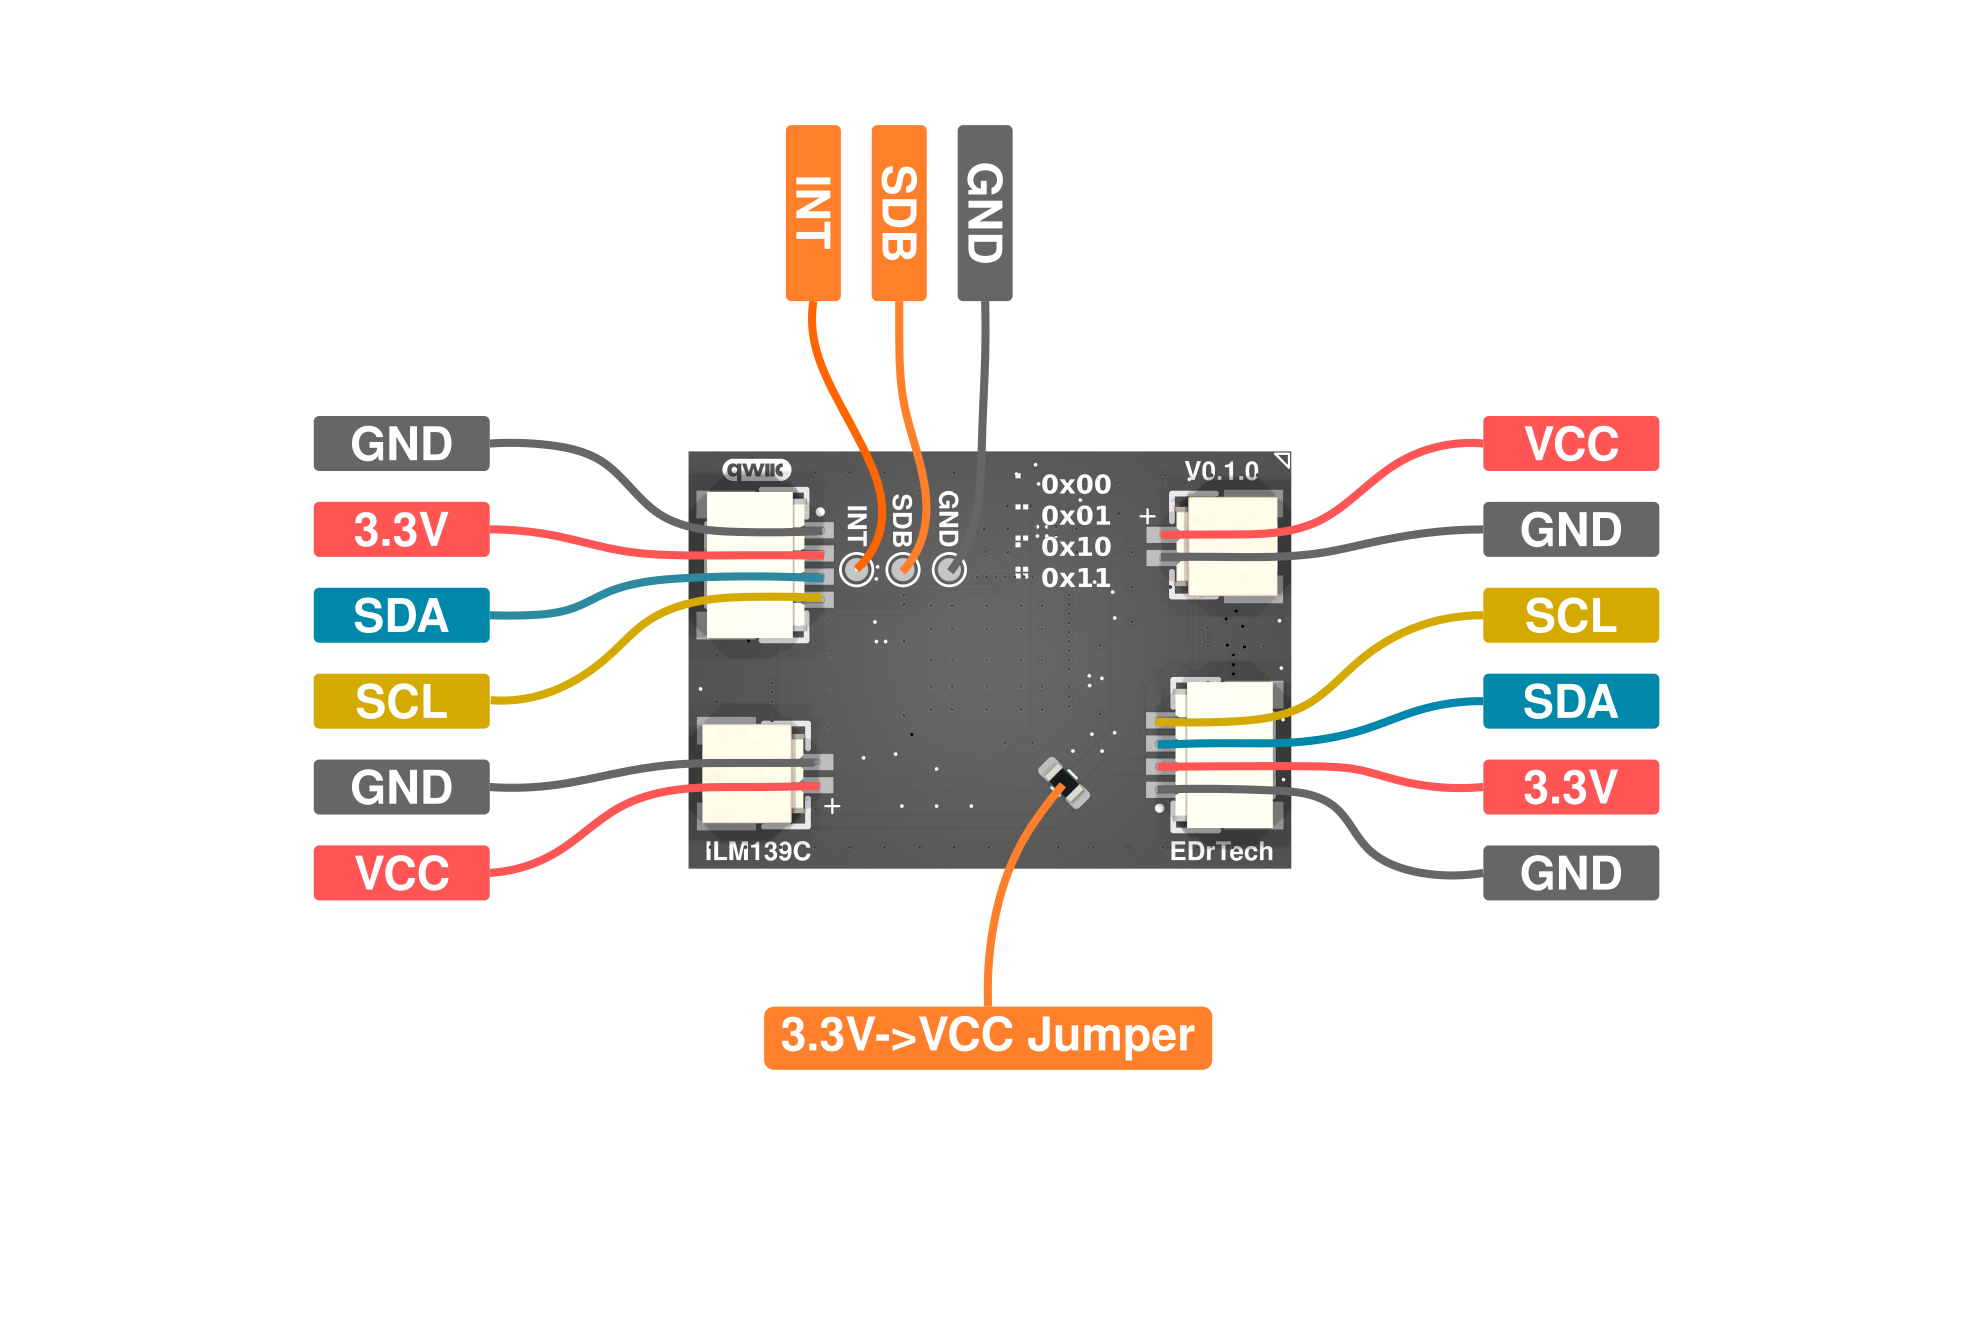
\includegraphics[width=450px]{../visual/ILM139C_pinout.png}\captionof{figure}{Module Pins}\label{fig:component}
	\end{center}
	
	
	\sectionbreak
	
	\section{Specifications}\label{sec:specs}
	\subsection{Absolute Maximum Ratings}\label{sec:specs.1}
	\begin{tabularx}{\textwidth}{|X|X|X|}
		\hline
		\rowcolor{gray!25}\textbf{PARAMETER} & \textbf{MAX RATING} & \textbf{UNIT} \\ \hline
		Supply Voltage (VCC) & 6.0 & V \\ \hline
		Storage Temperature & -40 to 85 & °C \\ \hline
	\end{tabularx}
	\captionof{table}{Absolute Maximum Ratings}\label{tab:amax}
	
	\subsection{Recommended Operating Conditions}\label{sec:specs.2}
	\begin{tabularx}{\textwidth}{|X|X|X|}
		\hline
		\rowcolor{gray!25}\textbf{PARAMETER} & \textbf{TYPICAL} & \textbf{UNIT} \\ \hline
		Input Voltage & 3.3 – 5.0 & V \\ \hline
		Operating Temp. Range & -20 to +70 & °C \\ \hline
	\end{tabularx}
	\captionof{table}{Recommended Operating Conditions}\label{tab:opcond}
	
	\subsection{Electrical Characteristics}\label{sec:specs.3}
	\begin{tabularx}{\textwidth}{|X|X|X|}
		\hline
		\rowcolor{gray!25}\textbf{PARAMETER} & \textbf{TYPICAL} & \textbf{UNIT} \\ \hline
		I\textsuperscript{2}C Clock Rate & 1000 & kHz \\ \hline
		LED Current (adjustable) & 1–30 & mA \\ \hline
	\end{tabularx}
	\captionof{table}{Electrical Characteristics}\label{tab:elec}
	
	\sectionbreak
	
	\section{Feature Description}\label{sec:features_desc}
	\subsection{Modular Construction}
	The ILM139C is split into two boards, simplifying repairs and customization. The LED matrix board can be removed or replaced independently of the driver.
	
	\subsection{Qwiic Interface and Power Options}
	The Qwiic system provides a 4-pin JST-SH connector for quick daisy-chaining of I\textsuperscript{2}C devices. Power is typically supplied via Qwiic (3.3V). A solderable SMD jumper on the back of the driver board connects 3.3V from Qwiic to the VCC rail.
	
	\textbf{Important:} If the jumper is soldered, do not connect another external power supply to the 2-pin VCC/GND connector to avoid damaging the module.
	
	If you wish to use external power (3.3–5V), leave the jumper open and connect a regulated supply to the 2-pin header.
	
	\subsection{LED Control and Flexibility}
	Each LED can be controlled independently for color and brightness. The IS31FL3741A handles PWM, current control, and I\textsuperscript{2}C interfacing. For advanced settings, refer to the \underline{\href{https://www.lumissil.com/assets/pdf/core/IS31FL3741A_DS.pdf}{IS31FL3741A datasheet}}
	
	\sectionbreak
	
	\section{Getting Started}\label{sec:getting}
	\subsection{Using Arduino}
	To use ILM139C with Arduino:
	
	\begin{enumerate}
		\item Connect the Qwiic cable to your controller.
		\item Solder the SMD jumper on the ILM139CD driver board if using Qwiic power.
		\item Install the library: \texttt{https://example.com/ILM139C-Arduino}
		\item Upload the basic example sketch.
	\end{enumerate}
	
	\texttt{
		Wire.begin(); \\
		ILM139C.begin(); \\
		ILM139C.setPixel(5, 3, 255, 0, 0);
	}
	
	\sectionbreak
	
	\section{Part numbering Information}\label{sec:order}
	\begin{tabularx}{\textwidth}{|X|X|X|}
		\hline
		\rowcolor{gray!25}\textbf{PART NUMBER} & \textbf{ORDER CODE} & \textbf{DESCRIPTION} \\ \hline
		ILM139C & ILM139C-BASE & Full RGB Matrix Module \\ \hline
		ILM139CD & ILM139C-DRV & Driver Moduleonly \\ \hline
		ILM139CM & ILM139C-MTX & LED Matrix only \\ \hline
	\end{tabularx}
	\captionof{table}{Ordering Information}\label{tab:order}
	
\end{document}
